\documentclass[1p]{elsarticle_modified}
%\bibliographystyle{elsarticle-num}

%\usepackage[colorlinks]{hyperref}
%\usepackage{abbrmath_seonhwa} %\Abb, \Ascr, \Acal ,\Abf, \Afrak
\usepackage{amsfonts}
\usepackage{amssymb}
\usepackage{amsmath}
\usepackage{amsthm}
\usepackage{scalefnt}
\usepackage{amsbsy}
\usepackage{kotex}
\usepackage{caption}
\usepackage{subfig}
\usepackage{color}
\usepackage{graphicx}
\usepackage{xcolor} %% white, black, red, green, blue, cyan, magenta, yellow
\usepackage{float}
\usepackage{setspace}
\usepackage{hyperref}

\usepackage{tikz}
\usetikzlibrary{arrows}

\usepackage{multirow}
\usepackage{array} % fixed length table
\usepackage{hhline}

%%%%%%%%%%%%%%%%%%%%%
\makeatletter
\renewcommand*\env@matrix[1][\arraystretch]{%
	\edef\arraystretch{#1}%
	\hskip -\arraycolsep
	\let\@ifnextchar\new@ifnextchar
	\array{*\c@MaxMatrixCols c}}
\makeatother %https://tex.stackexchange.com/questions/14071/how-can-i-increase-the-line-spacing-in-a-matrix
%%%%%%%%%%%%%%%

\usepackage[normalem]{ulem}

\newcommand{\msout}[1]{\ifmmode\text{\sout{\ensuremath{#1}}}\else\sout{#1}\fi}
%SOURCE: \msout is \stkout macro in https://tex.stackexchange.com/questions/20609/strikeout-in-math-mode

\newcommand{\cancel}[1]{
	\ifmmode
	{\color{red}\msout{#1}}
	\else
	{\color{red}\sout{#1}}
	\fi
}

\newcommand{\add}[1]{
	{\color{blue}\uwave{#1}}
}

\newcommand{\replace}[2]{
	\ifmmode
	{\color{red}\msout{#1}}{\color{blue}\uwave{#2}}
	\else
	{\color{red}\sout{#1}}{\color{blue}\uwave{#2}}
	\fi
}

\newcommand{\Sol}{\mathcal{S}} %segment
\newcommand{\D}{D} %diagram
\newcommand{\A}{\mathcal{A}} %arc


%%%%%%%%%%%%%%%%%%%%%%%%%%%%%5 test

\def\sl{\operatorname{\textup{SL}}(2,\Cbb)}
\def\psl{\operatorname{\textup{PSL}}(2,\Cbb)}
\def\quan{\mkern 1mu \triangleright \mkern 1mu}

\theoremstyle{definition}
\newtheorem{thm}{Theorem}[section]
\newtheorem{prop}[thm]{Proposition}
\newtheorem{lem}[thm]{Lemma}
\newtheorem{ques}[thm]{Question}
\newtheorem{cor}[thm]{Corollary}
\newtheorem{defn}[thm]{Definition}
\newtheorem{exam}[thm]{Example}
\newtheorem{rmk}[thm]{Remark}
\newtheorem{alg}[thm]{Algorithm}

\newcommand{\I}{\sqrt{-1}}
\begin{document}

%\begin{frontmatter}
%
%\title{Boundary parabolic representations of knots up to 8 crossings}
%
%%% Group authors per affiliation:
%\author{Yunhi Cho} 
%\address{Department of Mathematics, University of Seoul, Seoul, Korea}
%\ead{yhcho@uos.ac.kr}
%
%
%\author{Seonhwa Kim} %\fnref{s_kim}}
%\address{Center for Geometry and Physics, Institute for Basic Science, Pohang, 37673, Korea}
%\ead{ryeona17@ibs.re.kr}
%
%\author{Hyuk Kim}
%\address{Department of Mathematical Sciences, Seoul National University, Seoul 08826, Korea}
%\ead{hyukkim@snu.ac.kr}
%
%\author{Seokbeom Yoon}
%\address{Department of Mathematical Sciences, Seoul National University, Seoul, 08826,  Korea}
%\ead{sbyoon15@snu.ac.kr}
%
%\begin{abstract}
%We find all boundary parabolic representation of knots up to 8 crossings.
%
%\end{abstract}
%\begin{keyword}
%    \MSC[2010] 57M25 
%\end{keyword}
%
%\end{frontmatter}

%\linenumbers
%\tableofcontents
%
\newcommand\colored[1]{\textcolor{white}{\rule[-0.35ex]{0.8em}{1.4ex}}\kern-0.8em\color{red} #1}%
%\newcommand\colored[1]{\textcolor{white}{ #1}\kern-2.17ex	\textcolor{white}{ #1}\kern-1.81ex	\textcolor{white}{ #1}\kern-2.15ex\color{red}#1	}

{\Large $\underline{12n_{0741}~(K12n_{0741})}$}

\setlength{\tabcolsep}{10pt}
\renewcommand{\arraystretch}{1.6}
\vspace{1cm}\begin{tabular}{m{100pt}>{\centering\arraybackslash}m{274pt}}
\multirow{5}{120pt}{
	\centering
	\includegraphics[width=112pt]{../../../GIT/diagram.site/Diagrams/png/2830_12n_0741.png}\\
\ \ \ A knot diagram\footnotemark}&
\allowdisplaybreaks
\textbf{Linearized knot diagam} \\
\cline{2-2}
 &
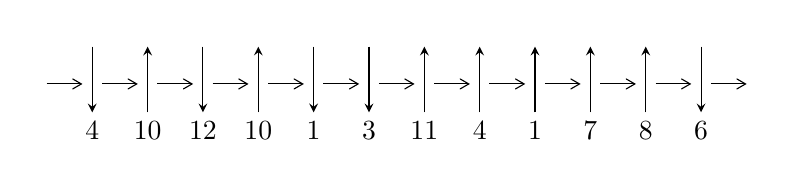
\begin{tikzpicture}[x=20pt, y=17pt]
	% nodes
	\node (C0) at (0, 0) {};
	\node (C1) at (1, 0) {};
	\node (C1U) at (1, +1) {};
	\node (C1D) at (1, -1) {4};

	\node (C2) at (2, 0) {};
	\node (C2U) at (2, +1) {};
	\node (C2D) at (2, -1) {10};

	\node (C3) at (3, 0) {};
	\node (C3U) at (3, +1) {};
	\node (C3D) at (3, -1) {12};

	\node (C4) at (4, 0) {};
	\node (C4U) at (4, +1) {};
	\node (C4D) at (4, -1) {10};

	\node (C5) at (5, 0) {};
	\node (C5U) at (5, +1) {};
	\node (C5D) at (5, -1) {1};

	\node (C6) at (6, 0) {};
	\node (C6U) at (6, +1) {};
	\node (C6D) at (6, -1) {3};

	\node (C7) at (7, 0) {};
	\node (C7U) at (7, +1) {};
	\node (C7D) at (7, -1) {11};

	\node (C8) at (8, 0) {};
	\node (C8U) at (8, +1) {};
	\node (C8D) at (8, -1) {4};

	\node (C9) at (9, 0) {};
	\node (C9U) at (9, +1) {};
	\node (C9D) at (9, -1) {1};

	\node (C10) at (10, 0) {};
	\node (C10U) at (10, +1) {};
	\node (C10D) at (10, -1) {7};

	\node (C11) at (11, 0) {};
	\node (C11U) at (11, +1) {};
	\node (C11D) at (11, -1) {8};

	\node (C12) at (12, 0) {};
	\node (C12U) at (12, +1) {};
	\node (C12D) at (12, -1) {6};
	\node (C13) at (13, 0) {};

	% arrows
	\draw[->,>={angle 60}]
	(C0) edge (C1) (C1) edge (C2) (C2) edge (C3) (C3) edge (C4) (C4) edge (C5) (C5) edge (C6) (C6) edge (C7) (C7) edge (C8) (C8) edge (C9) (C9) edge (C10) (C10) edge (C11) (C11) edge (C12) (C12) edge (C13) ;	\draw[->,>=stealth]
	(C1U) edge (C1D) (C2D) edge (C2U) (C3U) edge (C3D) (C4D) edge (C4U) (C5U) edge (C5D) (C6U) edge (C6D) (C7D) edge (C7U) (C8D) edge (C8U) (C9D) edge (C9U) (C10D) edge (C10U) (C11D) edge (C11U) (C12U) edge (C12D) ;
	\end{tikzpicture} \\
\hhline{~~} \\& 
\textbf{Solving Sequence} \\ \cline{2-2} 
 &
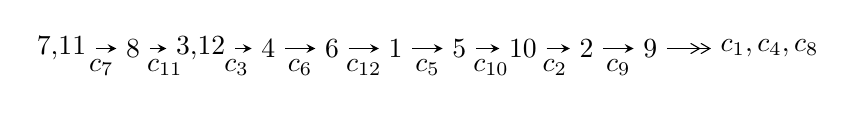
\begin{tikzpicture}[x=23pt, y=7pt]
	% node
	\node (A0) at (-1/8, 0) {7,11};
	\node (A1) at (1, 0) {8};
	\node (A2) at (33/16, 0) {3,12};
	\node (A3) at (25/8, 0) {4};
	\node (A4) at (33/8, 0) {6};
	\node (A5) at (41/8, 0) {1};
	\node (A6) at (49/8, 0) {5};
	\node (A7) at (57/8, 0) {10};
	\node (A8) at (65/8, 0) {2};
	\node (A9) at (73/8, 0) {9};
	\node (C1) at (1/2, -1) {$c_{7}$};
	\node (C2) at (3/2, -1) {$c_{11}$};
	\node (C3) at (21/8, -1) {$c_{3}$};
	\node (C4) at (29/8, -1) {$c_{6}$};
	\node (C5) at (37/8, -1) {$c_{12}$};
	\node (C6) at (45/8, -1) {$c_{5}$};
	\node (C7) at (53/8, -1) {$c_{10}$};
	\node (C8) at (61/8, -1) {$c_{2}$};
	\node (C9) at (69/8, -1) {$c_{9}$};
	\node (A10) at (11, 0) {$c_{1},c_{4},c_{8}$};

	% edge
	\draw[->,>=stealth]	
	(A0) edge (A1) (A1) edge (A2) (A2) edge (A3) (A3) edge (A4) (A4) edge (A5) (A5) edge (A6) (A6) edge (A7) (A7) edge (A8) (A8) edge (A9) ;
	\draw[->>,>={angle 60}]	
	(A9) edge (A10);
\end{tikzpicture} \\ 

\end{tabular} \\

\footnotetext{
The image of knot diagram is generated by the software ``\textbf{Draw programme}" developed by Andrew Bartholomew(\url{http://www.layer8.co.uk/maths/draw/index.htm\#Running-draw}), where we modified some parts for our purpose(\url{https://github.com/CATsTAILs/LinksPainter}).
}\phantom \\ \newline 
\centering \textbf{Ideals for irreducible components\footnotemark of $X_{\text{par}}$} 
 
\begin{align*}
I^u_{1}&=\langle 
-173 u^{29}-1170 u^{28}+\cdots+2 b+538,\;777 u^{29}+5170 u^{28}+\cdots+4 a-2260,\;u^{30}+8 u^{29}+\cdots+10 u-4\rangle \\
I^u_{2}&=\langle 
-8171 u^8 a^3+29276 u^8 a^2+\cdots-86275 a-355947,\;u^8 a^3+2 u^8 a^2+\cdots-6 a^2+20,\\
\phantom{I^u_{2}}&\phantom{= \langle  }u^9- u^8-4 u^7+3 u^6+5 u^5- u^4-2 u^3-2 u^2+u-1\rangle \\
I^u_{3}&=\langle 
-5 u^{18}+8 u^{17}+\cdots+b+4,\;12 u^{18}-20 u^{17}+\cdots+a-7,\;u^{19}-3 u^{18}+\cdots-3 u+1\rangle \\
\\
\end{align*}
\raggedright * 3 irreducible components of $\dim_{\mathbb{C}}=0$, with total 85 representations.\\
\footnotetext{All coefficients of polynomials are rational numbers. But the coefficients are sometimes approximated in decimal forms when there is not enough margin.}
\newpage
\renewcommand{\arraystretch}{1}
\centering \section*{I. $I^u_{1}= \langle -173 u^{29}-1170 u^{28}+\cdots+2 b+538,\;777 u^{29}+5170 u^{28}+\cdots+4 a-2260,\;u^{30}+8 u^{29}+\cdots+10 u-4 \rangle$}
\flushleft \textbf{(i) Arc colorings}\\
\begin{tabular}{m{7pt} m{180pt} m{7pt} m{180pt} }
\flushright $a_{7}=$&$\begin{pmatrix}1\\0\end{pmatrix}$ \\
\flushright $a_{11}=$&$\begin{pmatrix}0\\u\end{pmatrix}$ \\
\flushright $a_{8}=$&$\begin{pmatrix}1\\- u^2\end{pmatrix}$ \\
\flushright $a_{3}=$&$\begin{pmatrix}-\frac{777}{4} u^{29}-\frac{2585}{2} u^{28}+\cdots-\frac{7275}{4} u+565\\\frac{173}{2} u^{29}+585 u^{28}+\cdots+\frac{1769}{2} u-269\end{pmatrix}$ \\
\flushright $a_{12}=$&$\begin{pmatrix}u\\- u^3+u\end{pmatrix}$ \\
\flushright $a_{4}=$&$\begin{pmatrix}-\frac{349}{4} u^{29}-\frac{1127}{2} u^{28}+\cdots-\frac{2739}{4} u+219\\\frac{103}{2} u^{29}+321 u^{28}+\cdots+\frac{641}{2} u-107\end{pmatrix}$ \\
\flushright $a_{6}=$&$\begin{pmatrix}-62.5000 u^{29}-410.500 u^{28}+\cdots-545.500 u+172.500\\\frac{73}{2} u^{29}+244 u^{28}+\cdots+\frac{697}{2} u-108\end{pmatrix}$ \\
\flushright $a_{1}=$&$\begin{pmatrix}-\frac{73}{4} u^{29}-\frac{287}{2} u^{28}+\cdots-\frac{1355}{4} u+95\\-\frac{35}{2} u^{29}-99 u^{28}+\cdots-\frac{51}{2} u+17\end{pmatrix}$ \\
\flushright $a_{5}=$&$\begin{pmatrix}\frac{557}{4} u^{29}+\frac{1839}{2} u^{28}+\cdots+\frac{5051}{4} u-393\\-\frac{207}{2} u^{29}-677 u^{28}+\cdots-\frac{1797}{2} u+281\end{pmatrix}$ \\
\flushright $a_{10}=$&$\begin{pmatrix}- u\\u\end{pmatrix}$ \\
\flushright $a_{2}=$&$\begin{pmatrix}\frac{107}{4} u^{29}+\frac{325}{2} u^{28}+\cdots+\frac{629}{4} u-53\\-\frac{269}{2} u^{29}-870 u^{28}+\cdots-\frac{2183}{2} u+349\end{pmatrix}$ \\
\flushright $a_{9}=$&$\begin{pmatrix}-36.5000 u^{29}-249.500 u^{28}+\cdots-394.500 u+120.500\\\frac{71}{2} u^{29}+241 u^{28}+\cdots+\frac{747}{2} u-114\end{pmatrix}$\\&\end{tabular}
\flushleft \textbf{(ii) Obstruction class $= -1$}\\~\\
\flushleft \textbf{(iii) Cusp Shapes $= 144 u^{29}+932 u^{28}+1166 u^{27}-3950 u^{26}-8068 u^{25}+10520 u^{24}+22058 u^{23}-31648 u^{22}-41053 u^{21}+75734 u^{20}+35810 u^{19}-138024 u^{18}+30849 u^{17}+178037 u^{16}-127069 u^{15}-106576 u^{14}+194708 u^{13}-23158 u^{12}-141581 u^{11}+93195 u^{10}+10441 u^9-78959 u^8+26181 u^7-2885 u^6-24227 u^5+9152 u^4-1810 u^3-3043 u^2+1148 u-374$}\\~\\
\newpage\renewcommand{\arraystretch}{1}
\flushleft \textbf{(iv) u-Polynomials at the component}\newline \\
\begin{tabular}{m{50pt}|m{274pt}}
Crossings & \hspace{64pt}u-Polynomials at each crossing \\
\hline $$\begin{aligned}c_{1}\end{aligned}$$&$\begin{aligned}
&u^{30}-20 u^{29}+\cdots+4520 u-448
\end{aligned}$\\
\hline $$\begin{aligned}c_{2},c_{8}\end{aligned}$$&$\begin{aligned}
&u^{30}+u^{29}+\cdots-24 u+5
\end{aligned}$\\
\hline $$\begin{aligned}c_{3},c_{6}\end{aligned}$$&$\begin{aligned}
&u^{30}- u^{29}+\cdots+12 u-1
\end{aligned}$\\
\hline $$\begin{aligned}c_{4},c_{9}\end{aligned}$$&$\begin{aligned}
&u^{30}+20 u^{28}+\cdots- u+1
\end{aligned}$\\
\hline $$\begin{aligned}c_{5},c_{12}\end{aligned}$$&$\begin{aligned}
&u^{30}+20 u^{29}+\cdots-6144 u-512
\end{aligned}$\\
\hline $$\begin{aligned}c_{7},c_{10},c_{11}\end{aligned}$$&$\begin{aligned}
&u^{30}-8 u^{29}+\cdots-10 u-4
\end{aligned}$\\
\hline
\end{tabular}\\~\\
\newpage\renewcommand{\arraystretch}{1}
\flushleft \textbf{(v) Riley Polynomials at the component}\newline \\
\begin{tabular}{m{50pt}|m{274pt}}
Crossings & \hspace{64pt}Riley Polynomials at each crossing \\
\hline $$\begin{aligned}c_{1}\end{aligned}$$&$\begin{aligned}
&y^{30}-16 y^{29}+\cdots-8229568 y+200704
\end{aligned}$\\
\hline $$\begin{aligned}c_{2},c_{8}\end{aligned}$$&$\begin{aligned}
&y^{30}-3 y^{29}+\cdots-256 y+25
\end{aligned}$\\
\hline $$\begin{aligned}c_{3},c_{6}\end{aligned}$$&$\begin{aligned}
&y^{30}+7 y^{29}+\cdots-80 y+1
\end{aligned}$\\
\hline $$\begin{aligned}c_{4},c_{9}\end{aligned}$$&$\begin{aligned}
&y^{30}+40 y^{29}+\cdots+9 y+1
\end{aligned}$\\
\hline $$\begin{aligned}c_{5},c_{12}\end{aligned}$$&$\begin{aligned}
&y^{30}+14 y^{29}+\cdots-3407872 y+262144
\end{aligned}$\\
\hline $$\begin{aligned}c_{7},c_{10},c_{11}\end{aligned}$$&$\begin{aligned}
&y^{30}-28 y^{29}+\cdots+100 y+16
\end{aligned}$\\
\hline
\end{tabular}\\~\\
\newpage\flushleft \textbf{(vi) Complex Volumes and Cusp Shapes}
$$\begin{array}{c|c|c}  
\text{Solutions to }I^u_{1}& \I (\text{vol} + \sqrt{-1}CS) & \text{Cusp shape}\\
 \hline 
\begin{aligned}
u &= \phantom{-}0.727622 + 0.705125 I \\
a &= -0.641027 + 0.115701 I \\
b &= \phantom{-}0.687397 + 1.021870 I\end{aligned}
 & -2.97556 - 6.23052 I & \phantom{-}3.26934 + 3.73627 I \\ \hline\begin{aligned}
u &= \phantom{-}0.727622 - 0.705125 I \\
a &= -0.641027 - 0.115701 I \\
b &= \phantom{-}0.687397 - 1.021870 I\end{aligned}
 & -2.97556 + 6.23052 I & \phantom{-}3.26934 - 3.73627 I \\ \hline\begin{aligned}
u &= \phantom{-}0.407170 + 0.935936 I \\
a &= -0.438010 - 0.324040 I \\
b &= -0.682979 + 0.645597 I\end{aligned}
 & -7.02127 + 3.79327 I & \phantom{-}0.05806 - 6.52210 I \\ \hline\begin{aligned}
u &= \phantom{-}0.407170 - 0.935936 I \\
a &= -0.438010 + 0.324040 I \\
b &= -0.682979 - 0.645597 I\end{aligned}
 & -7.02127 - 3.79327 I & \phantom{-}0.05806 + 6.52210 I \\ \hline\begin{aligned}
u &= \phantom{-}0.427689 + 0.823483 I \\
a &= \phantom{-}0.796629 + 0.599604 I \\
b &= \phantom{-}0.96991 - 1.17666 I\end{aligned}
 & -3.86787 + 11.40560 I & \phantom{-}1.94326 - 7.48134 I \\ \hline\begin{aligned}
u &= \phantom{-}0.427689 - 0.823483 I \\
a &= \phantom{-}0.796629 - 0.599604 I \\
b &= \phantom{-}0.96991 + 1.17666 I\end{aligned}
 & -3.86787 - 11.40560 I & \phantom{-}1.94326 + 7.48134 I \\ \hline\begin{aligned}
u &= \phantom{-}1.005300 + 0.779911 I \\
a &= \phantom{-}0.231346 + 0.022494 I \\
b &= -0.272840 - 0.574864 I\end{aligned}
 & -5.41208 + 2.17475 I & \phantom{-}9.73919 + 5.03605 I \\ \hline\begin{aligned}
u &= \phantom{-}1.005300 - 0.779911 I \\
a &= \phantom{-}0.231346 - 0.022494 I \\
b &= -0.272840 + 0.574864 I\end{aligned}
 & -5.41208 - 2.17475 I & \phantom{-}9.73919 - 5.03605 I \\ \hline\begin{aligned}
u &= \phantom{-}1.313940 + 0.059506 I \\
a &= \phantom{-}0.372373 - 0.163949 I \\
b &= -1.166230 + 0.417498 I\end{aligned}
 & \phantom{-}5.91755 + 3.45804 I & \phantom{-}11.41104 - 3.47795 I \\ \hline\begin{aligned}
u &= \phantom{-}1.313940 - 0.059506 I \\
a &= \phantom{-}0.372373 + 0.163949 I \\
b &= -1.166230 - 0.417498 I\end{aligned}
 & \phantom{-}5.91755 - 3.45804 I & \phantom{-}11.41104 + 3.47795 I\\
 \hline 
 \end{array}$$\newpage$$\begin{array}{c|c|c}  
\text{Solutions to }I^u_{1}& \I (\text{vol} + \sqrt{-1}CS) & \text{Cusp shape}\\
 \hline 
\begin{aligned}
u &= \phantom{-}1.31986\phantom{ +0.000000I} \\
a &= -0.423063\phantom{ +0.000000I} \\
b &= \phantom{-}1.29538\phantom{ +0.000000I}\end{aligned}
 & \phantom{-}2.18151\phantom{ +0.000000I} & \phantom{-}4.39970\phantom{ +0.000000I} \\ \hline\begin{aligned}
u &= -0.654747\phantom{ +0.000000I} \\
a &= -0.472043\phantom{ +0.000000I} \\
b &= -0.106707\phantom{ +0.000000I}\end{aligned}
 & \phantom{-}0.896294\phantom{ +0.000000I} & \phantom{-}12.8060\phantom{ +0.000000I} \\ \hline\begin{aligned}
u &= \phantom{-}0.039034 + 0.641181 I \\
a &= \phantom{-}0.279594 - 0.811369 I \\
b &= -0.457242 - 0.493923 I\end{aligned}
 & \phantom{-}2.19604 - 1.41771 I & \phantom{-}2.97939 + 4.71269 I \\ \hline\begin{aligned}
u &= \phantom{-}0.039034 - 0.641181 I \\
a &= \phantom{-}0.279594 + 0.811369 I \\
b &= -0.457242 + 0.493923 I\end{aligned}
 & \phantom{-}2.19604 + 1.41771 I & \phantom{-}2.97939 - 4.71269 I \\ \hline\begin{aligned}
u &= -1.359280 + 0.360594 I \\
a &= \phantom{-}0.830579 - 0.466140 I \\
b &= -0.008753 + 0.681742 I\end{aligned}
 & \phantom{-}6.54442 - 2.48074 I & \phantom{-}9.12565 + 0. I\phantom{ +0.000000I} \\ \hline\begin{aligned}
u &= -1.359280 - 0.360594 I \\
a &= \phantom{-}0.830579 + 0.466140 I \\
b &= -0.008753 - 0.681742 I\end{aligned}
 & \phantom{-}6.54442 + 2.48074 I & \phantom{-}9.12565 + 0. I\phantom{ +0.000000I} \\ \hline\begin{aligned}
u &= -1.41614 + 0.09837 I \\
a &= -0.21812 - 1.68007 I \\
b &= \phantom{-}0.429262 + 0.934517 I\end{aligned}
 & \phantom{-}4.01008 - 2.17507 I & \phantom{-0.000000 } 0 \\ \hline\begin{aligned}
u &= -1.41614 - 0.09837 I \\
a &= -0.21812 + 1.68007 I \\
b &= \phantom{-}0.429262 - 0.934517 I\end{aligned}
 & \phantom{-}4.01008 + 2.17507 I & \phantom{-0.000000 } 0 \\ \hline\begin{aligned}
u &= -1.43489 + 0.15441 I \\
a &= \phantom{-}0.22751 + 2.33475 I \\
b &= -0.81061 - 1.33560 I\end{aligned}
 & \phantom{-}9.21909 - 5.77084 I & \phantom{-0.000000 } 0 \\ \hline\begin{aligned}
u &= -1.43489 - 0.15441 I \\
a &= \phantom{-}0.22751 - 2.33475 I \\
b &= -0.81061 + 1.33560 I\end{aligned}
 & \phantom{-}9.21909 + 5.77084 I & \phantom{-0.000000 } 0\\
 \hline 
 \end{array}$$\newpage$$\begin{array}{c|c|c}  
\text{Solutions to }I^u_{1}& \I (\text{vol} + \sqrt{-1}CS) & \text{Cusp shape}\\
 \hline 
\begin{aligned}
u &= \phantom{-}0.340842 + 0.386198 I \\
a &= -0.70853 - 1.64819 I \\
b &= -0.852307 + 0.967588 I\end{aligned}
 & \phantom{-}3.46376 + 3.69110 I & -2.17441 - 2.03577 I \\ \hline\begin{aligned}
u &= \phantom{-}0.340842 - 0.386198 I \\
a &= -0.70853 + 1.64819 I \\
b &= -0.852307 - 0.967588 I\end{aligned}
 & \phantom{-}3.46376 - 3.69110 I & -2.17441 + 2.03577 I \\ \hline\begin{aligned}
u &= -1.49409 + 0.30547 I \\
a &= \phantom{-}0.16084 - 1.98951 I \\
b &= \phantom{-}1.10456 + 1.38075 I\end{aligned}
 & \phantom{-}2.3325 - 15.5061 I & \phantom{-0.000000 } 0 \\ \hline\begin{aligned}
u &= -1.49409 - 0.30547 I \\
a &= \phantom{-}0.16084 + 1.98951 I \\
b &= \phantom{-}1.10456 - 1.38075 I\end{aligned}
 & \phantom{-}2.3325 + 15.5061 I & \phantom{-0.000000 } 0 \\ \hline\begin{aligned}
u &= -1.49706 + 0.34161 I \\
a &= -0.064520 + 1.358570 I \\
b &= -0.885003 - 0.896360 I\end{aligned}
 & -0.89522 - 8.36672 I & \phantom{-0.000000 } 0 \\ \hline\begin{aligned}
u &= -1.49706 - 0.34161 I \\
a &= -0.064520 - 1.358570 I \\
b &= -0.885003 + 0.896360 I\end{aligned}
 & -0.89522 + 8.36672 I & \phantom{-0.000000 } 0 \\ \hline\begin{aligned}
u &= -1.57559 + 0.10910 I \\
a &= -0.517743 + 1.206130 I \\
b &= \phantom{-}0.180303 - 1.201000 I\end{aligned}
 & \phantom{-}5.04077 + 3.42733 I & \phantom{-0.000000 } 0 \\ \hline\begin{aligned}
u &= -1.57559 - 0.10910 I \\
a &= -0.517743 - 1.206130 I \\
b &= \phantom{-}0.180303 + 1.201000 I\end{aligned}
 & \phantom{-}5.04077 - 3.42733 I & \phantom{-0.000000 } 0 \\ \hline\begin{aligned}
u &= \phantom{-}0.182909 + 0.333059 I \\
a &= \phantom{-}0.38663 + 1.56291 I \\
b &= \phantom{-}0.670201 - 0.340664 I\end{aligned}
 & -1.174400 + 0.676840 I & -4.63993 - 2.36566 I \\ \hline\begin{aligned}
u &= \phantom{-}0.182909 - 0.333059 I \\
a &= \phantom{-}0.38663 - 1.56291 I \\
b &= \phantom{-}0.670201 + 0.340664 I\end{aligned}
 & -1.174400 - 0.676840 I & -4.63993 + 2.36566 I\\
 \hline 
 \end{array}$$\newpage\newpage\renewcommand{\arraystretch}{1}
\centering \section*{II. $I^u_{2}= \langle -8171 a^{3} u^{8}+2.93\times10^{4} a^{2} u^{8}+\cdots-8.63\times10^{4} a-3.56\times10^{5},\;u^8 a^3+2 u^8 a^2+\cdots-6 a^2+20,\;u^9- u^8+\cdots+u-1 \rangle$}
\flushleft \textbf{(i) Arc colorings}\\
\begin{tabular}{m{7pt} m{180pt} m{7pt} m{180pt} }
\flushright $a_{7}=$&$\begin{pmatrix}1\\0\end{pmatrix}$ \\
\flushright $a_{11}=$&$\begin{pmatrix}0\\u\end{pmatrix}$ \\
\flushright $a_{8}=$&$\begin{pmatrix}1\\- u^2\end{pmatrix}$ \\
\flushright $a_{3}=$&$\begin{pmatrix}a\\0.0368350 a^{3} u^{8}-0.131977 a^{2} u^{8}+\cdots+0.388929 a+1.60462\end{pmatrix}$ \\
\flushright $a_{12}=$&$\begin{pmatrix}u\\- u^3+u\end{pmatrix}$ \\
\flushright $a_{4}=$&$\begin{pmatrix}-0.0970216 a^{3} u^{8}-0.329653 a^{2} u^{8}+\cdots+0.730934 a-0.927002\\0.349200 a^{3} u^{8}+0.466016 a^{2} u^{8}+\cdots+0.921213 a+2.65521\end{pmatrix}$ \\
\flushright $a_{6}=$&$\begin{pmatrix}0.0154895 a^{3} u^{8}+0.0725160 a^{2} u^{8}+\cdots+0.0316192 a+1.77573\\-0.451609 a^{3} u^{8}-0.579330 a^{2} u^{8}+\cdots-0.740857 a-1.41865\end{pmatrix}$ \\
\flushright $a_{1}=$&$\begin{pmatrix}0.182183 a^{3} u^{8}+0.0979592 a^{2} u^{8}+\cdots-0.599584 a+1.10198\\-0.416915 a^{3} u^{8}-0.0688284 a^{2} u^{8}+\cdots-2.38249 a-2.38081\end{pmatrix}$ \\
\flushright $a_{5}=$&$\begin{pmatrix}0.261826 a^{3} u^{8}+0.0418299 a^{2} u^{8}+\cdots-0.0522569 a+0.418560\\-0.514004 a^{3} u^{8}-0.178193 a^{2} u^{8}+\cdots-1.59989 a-2.14677\end{pmatrix}$ \\
\flushright $a_{10}=$&$\begin{pmatrix}- u\\u\end{pmatrix}$ \\
\flushright $a_{2}=$&$\begin{pmatrix}-0.0970216 a^{3} u^{8}-0.329653 a^{2} u^{8}+\cdots+0.730934 a-0.927002\\0.133857 a^{3} u^{8}+0.197677 a^{2} u^{8}+\cdots+0.657995 a+2.53162\end{pmatrix}$ \\
\flushright $a_{9}=$&$\begin{pmatrix}0.235697 a^{3} u^{8}-0.0385841 a^{2} u^{8}+\cdots-0.288364 a-1.35213\\-0.0885780 a^{3} u^{8}+0.0969539 a^{2} u^{8}+\cdots-2.45381 a+2.63002\end{pmatrix}$\\&\end{tabular}
\flushleft \textbf{(ii) Obstruction class $= -1$}\\~\\
\flushleft \textbf{(iii) Cusp Shapes $= \frac{156832}{221827} u^8 a^3+\frac{113420}{221827} u^8 a^2+\cdots+\frac{193092}{221827} a-\frac{704302}{221827}$}\\~\\
\newpage\renewcommand{\arraystretch}{1}
\flushleft \textbf{(iv) u-Polynomials at the component}\newline \\
\begin{tabular}{m{50pt}|m{274pt}}
Crossings & \hspace{64pt}u-Polynomials at each crossing \\
\hline $$\begin{aligned}c_{1}\end{aligned}$$&$\begin{aligned}
&(u^9+7 u^8+16 u^7+7 u^6-19 u^5-11 u^4+20 u^3+6 u^2-11 u+3)^4
\end{aligned}$\\
\hline $$\begin{aligned}c_{2},c_{8}\end{aligned}$$&$\begin{aligned}
&u^{36}- u^{35}+\cdots-8292 u+619
\end{aligned}$\\
\hline $$\begin{aligned}c_{3},c_{6}\end{aligned}$$&$\begin{aligned}
&u^{36}+7 u^{35}+\cdots+244 u+193
\end{aligned}$\\
\hline $$\begin{aligned}c_{4},c_{9}\end{aligned}$$&$\begin{aligned}
&u^{36}- u^{35}+\cdots-520 u+2089
\end{aligned}$\\
\hline $$\begin{aligned}c_{5},c_{12}\end{aligned}$$&$\begin{aligned}
&(u^2- u+1)^{18}
\end{aligned}$\\
\hline $$\begin{aligned}c_{7},c_{10},c_{11}\end{aligned}$$&$\begin{aligned}
&(u^9+u^8-4 u^7-3 u^6+5 u^5+u^4-2 u^3+2 u^2+u+1)^4
\end{aligned}$\\
\hline
\end{tabular}\\~\\
\newpage\renewcommand{\arraystretch}{1}
\flushleft \textbf{(v) Riley Polynomials at the component}\newline \\
\begin{tabular}{m{50pt}|m{274pt}}
Crossings & \hspace{64pt}Riley Polynomials at each crossing \\
\hline $$\begin{aligned}c_{1}\end{aligned}$$&$\begin{aligned}
&(y^9-17 y^8+\cdots+85 y-9)^{4}
\end{aligned}$\\
\hline $$\begin{aligned}c_{2},c_{8}\end{aligned}$$&$\begin{aligned}
&y^{36}+11 y^{35}+\cdots-41360324 y+383161
\end{aligned}$\\
\hline $$\begin{aligned}c_{3},c_{6}\end{aligned}$$&$\begin{aligned}
&y^{36}+11 y^{35}+\cdots-118980 y+37249
\end{aligned}$\\
\hline $$\begin{aligned}c_{4},c_{9}\end{aligned}$$&$\begin{aligned}
&y^{36}+35 y^{35}+\cdots+136249928 y+4363921
\end{aligned}$\\
\hline $$\begin{aligned}c_{5},c_{12}\end{aligned}$$&$\begin{aligned}
&(y^2+y+1)^{18}
\end{aligned}$\\
\hline $$\begin{aligned}c_{7},c_{10},c_{11}\end{aligned}$$&$\begin{aligned}
&(y^9-9 y^8+32 y^7-55 y^6+45 y^5-19 y^4+16 y^3-10 y^2-3 y-1)^4
\end{aligned}$\\
\hline
\end{tabular}\\~\\
\newpage\flushleft \textbf{(vi) Complex Volumes and Cusp Shapes}
$$\begin{array}{c|c|c}  
\text{Solutions to }I^u_{2}& \I (\text{vol} + \sqrt{-1}CS) & \text{Cusp shape}\\
 \hline 
\begin{aligned}
u &= -0.482242 + 0.666986 I \\
a &= -0.829276 - 0.258734 I \\
b &= \phantom{-}0.030585 - 0.881502 I\end{aligned}
 & \phantom{-}2.12882 - 0.18400 I & \phantom{-}2.24115 - 0.41812 I \\ \hline\begin{aligned}
u &= -0.482242 + 0.666986 I \\
a &= -0.693533 + 0.971150 I \\
b &= -0.702014 - 0.777525 I\end{aligned}
 & \phantom{-}2.12882 - 4.24376 I & \phantom{-}2.24115 + 6.51008 I \\ \hline\begin{aligned}
u &= -0.482242 + 0.666986 I \\
a &= \phantom{-}0.579089 - 0.313786 I \\
b &= \phantom{-}0.638098 + 1.236810 I\end{aligned}
 & \phantom{-}2.12882 - 4.24376 I & \phantom{-}2.24115 + 6.51008 I \\ \hline\begin{aligned}
u &= -0.482242 + 0.666986 I \\
a &= \phantom{-}0.317204 - 0.169060 I \\
b &= -0.396381 + 0.596506 I\end{aligned}
 & \phantom{-}2.12882 - 0.18400 I & \phantom{-}2.24115 - 0.41812 I \\ \hline\begin{aligned}
u &= -0.482242 - 0.666986 I \\
a &= -0.829276 + 0.258734 I \\
b &= \phantom{-}0.030585 + 0.881502 I\end{aligned}
 & \phantom{-}2.12882 + 0.18400 I & \phantom{-}2.24115 + 0.41812 I \\ \hline\begin{aligned}
u &= -0.482242 - 0.666986 I \\
a &= -0.693533 - 0.971150 I \\
b &= -0.702014 + 0.777525 I\end{aligned}
 & \phantom{-}2.12882 + 4.24376 I & \phantom{-}2.24115 - 6.51008 I \\ \hline\begin{aligned}
u &= -0.482242 - 0.666986 I \\
a &= \phantom{-}0.579089 + 0.313786 I \\
b &= \phantom{-}0.638098 - 1.236810 I\end{aligned}
 & \phantom{-}2.12882 + 4.24376 I & \phantom{-}2.24115 - 6.51008 I \\ \hline\begin{aligned}
u &= -0.482242 - 0.666986 I \\
a &= \phantom{-}0.317204 + 0.169060 I \\
b &= -0.396381 - 0.596506 I\end{aligned}
 & \phantom{-}2.12882 + 0.18400 I & \phantom{-}2.24115 + 0.41812 I \\ \hline\begin{aligned}
u &= \phantom{-}1.28056\phantom{ +0.000000I} \\
a &= \phantom{-}0.24822 + 2.48346 I \\
b &= \phantom{-}0.425790 - 0.000287 I\end{aligned}
 & -2.09801 + 2.02988 I & -0.33330 - 3.46410 I \\ \hline\begin{aligned}
u &= \phantom{-}1.28056\phantom{ +0.000000I} \\
a &= \phantom{-}0.24822 - 2.48346 I \\
b &= \phantom{-}0.425790 + 0.000287 I\end{aligned}
 & -2.09801 - 2.02988 I & -0.33330 + 3.46410 I\\
 \hline 
 \end{array}$$\newpage$$\begin{array}{c|c|c}  
\text{Solutions to }I^u_{2}& \I (\text{vol} + \sqrt{-1}CS) & \text{Cusp shape}\\
 \hline 
\begin{aligned}
u &= \phantom{-}1.28056\phantom{ +0.000000I} \\
a &= -0.65036 + 3.17999 I \\
b &= \phantom{-}0.74862 - 2.03443 I\end{aligned}
 & -2.09801 - 2.02988 I & -0.33330 + 3.46410 I \\ \hline\begin{aligned}
u &= \phantom{-}1.28056\phantom{ +0.000000I} \\
a &= -0.65036 - 3.17999 I \\
b &= \phantom{-}0.74862 + 2.03443 I\end{aligned}
 & -2.09801 + 2.02988 I & -0.33330 - 3.46410 I \\ \hline\begin{aligned}
u &= -1.380230 + 0.162431 I \\
a &= -1.051670 + 0.187613 I \\
b &= -0.693072 - 0.293619 I\end{aligned}
 & \phantom{-}0.22800 - 5.44061 I & \phantom{-}3.88238 + 7.86053 I \\ \hline\begin{aligned}
u &= -1.380230 + 0.162431 I \\
a &= \phantom{-}0.207018 - 1.238430 I \\
b &= \phantom{-}1.253150 + 0.213191 I\end{aligned}
 & \phantom{-}0.227995 - 1.380850 I & \phantom{-}3.88238 + 0.93232 I \\ \hline\begin{aligned}
u &= -1.380230 + 0.162431 I \\
a &= \phantom{-}0.96217 - 1.48521 I \\
b &= -1.05706 + 1.47865 I\end{aligned}
 & \phantom{-}0.227995 - 1.380850 I & \phantom{-}3.88238 + 0.93232 I \\ \hline\begin{aligned}
u &= -1.380230 + 0.162431 I \\
a &= -1.89166 + 0.16166 I \\
b &= \phantom{-}2.06020 - 0.72212 I\end{aligned}
 & \phantom{-}0.22800 - 5.44061 I & \phantom{-}3.88238 + 7.86053 I \\ \hline\begin{aligned}
u &= -1.380230 - 0.162431 I \\
a &= -1.051670 - 0.187613 I \\
b &= -0.693072 + 0.293619 I\end{aligned}
 & \phantom{-}0.22800 + 5.44061 I & \phantom{-}3.88238 - 7.86053 I \\ \hline\begin{aligned}
u &= -1.380230 - 0.162431 I \\
a &= \phantom{-}0.207018 + 1.238430 I \\
b &= \phantom{-}1.253150 - 0.213191 I\end{aligned}
 & \phantom{-}0.227995 + 1.380850 I & \phantom{-}3.88238 - 0.93232 I \\ \hline\begin{aligned}
u &= -1.380230 - 0.162431 I \\
a &= \phantom{-}0.96217 + 1.48521 I \\
b &= -1.05706 - 1.47865 I\end{aligned}
 & \phantom{-}0.227995 + 1.380850 I & \phantom{-}3.88238 - 0.93232 I \\ \hline\begin{aligned}
u &= -1.380230 - 0.162431 I \\
a &= -1.89166 - 0.16166 I \\
b &= \phantom{-}2.06020 + 0.72212 I\end{aligned}
 & \phantom{-}0.22800 + 5.44061 I & \phantom{-}3.88238 - 7.86053 I\\
 \hline 
 \end{array}$$\newpage$$\begin{array}{c|c|c}  
\text{Solutions to }I^u_{2}& \I (\text{vol} + \sqrt{-1}CS) & \text{Cusp shape}\\
 \hline 
\begin{aligned}
u &= \phantom{-}0.230908 + 0.456719 I \\
a &= -0.700916 + 0.499752 I \\
b &= -0.37028 - 1.40207 I\end{aligned}
 & -4.89942 - 0.92019 I & -1.44626 - 2.77537 I \\ \hline\begin{aligned}
u &= \phantom{-}0.230908 + 0.456719 I \\
a &= \phantom{-}0.730726 + 0.224850 I \\
b &= \phantom{-}1.44747 + 0.99796 I\end{aligned}
 & -4.89942 + 3.13958 I & -1.44626 - 9.70357 I \\ \hline\begin{aligned}
u &= \phantom{-}0.230908 + 0.456719 I \\
a &= \phantom{-}3.16147 + 0.79514 I \\
b &= \phantom{-}1.048700 - 0.338629 I\end{aligned}
 & -4.89942 - 0.92019 I & -1.44626 - 2.77537 I \\ \hline\begin{aligned}
u &= \phantom{-}0.230908 + 0.456719 I \\
a &= -3.08241 + 1.25861 I \\
b &= -0.279189 + 0.459914 I\end{aligned}
 & -4.89942 + 3.13958 I & -1.44626 - 9.70357 I \\ \hline\begin{aligned}
u &= \phantom{-}0.230908 - 0.456719 I \\
a &= -0.700916 - 0.499752 I \\
b &= -0.37028 + 1.40207 I\end{aligned}
 & -4.89942 + 0.92019 I & -1.44626 + 2.77537 I \\ \hline\begin{aligned}
u &= \phantom{-}0.230908 - 0.456719 I \\
a &= \phantom{-}0.730726 - 0.224850 I \\
b &= \phantom{-}1.44747 - 0.99796 I\end{aligned}
 & -4.89942 - 3.13958 I & -1.44626 + 9.70357 I \\ \hline\begin{aligned}
u &= \phantom{-}0.230908 - 0.456719 I \\
a &= \phantom{-}3.16147 - 0.79514 I \\
b &= \phantom{-}1.048700 + 0.338629 I\end{aligned}
 & -4.89942 + 0.92019 I & -1.44626 + 2.77537 I \\ \hline\begin{aligned}
u &= \phantom{-}0.230908 - 0.456719 I \\
a &= -3.08241 - 1.25861 I \\
b &= -0.279189 - 0.459914 I\end{aligned}
 & -4.89942 - 3.13958 I & -1.44626 + 9.70357 I \\ \hline\begin{aligned}
u &= \phantom{-}1.49128 + 0.23430 I \\
a &= \phantom{-}0.510760 + 1.162850 I \\
b &= -0.059502 - 0.853778 I\end{aligned}
 & \phantom{-}8.52641 + 3.47060 I & \phantom{-}5.48937 + 0.49112 I \\ \hline\begin{aligned}
u &= \phantom{-}1.49128 + 0.23430 I \\
a &= -0.362517 - 1.301200 I \\
b &= -0.612207 + 1.221860 I\end{aligned}
 & \phantom{-}8.52641 + 3.47060 I & \phantom{-}5.48937 + 0.49112 I\\
 \hline 
 \end{array}$$\newpage$$\begin{array}{c|c|c}  
\text{Solutions to }I^u_{2}& \I (\text{vol} + \sqrt{-1}CS) & \text{Cusp shape}\\
 \hline 
\begin{aligned}
u &= \phantom{-}1.49128 + 0.23430 I \\
a &= -0.11348 - 1.82407 I \\
b &= -0.792237 + 0.983649 I\end{aligned}
 & \phantom{-}8.52641 + 7.53037 I & \phantom{-}5.48937 - 6.43708 I \\ \hline\begin{aligned}
u &= \phantom{-}1.49128 + 0.23430 I \\
a &= \phantom{-}0.15917 + 2.02163 I \\
b &= \phantom{-}0.80933 - 1.74941 I\end{aligned}
 & \phantom{-}8.52641 + 7.53037 I & \phantom{-}5.48937 - 6.43708 I \\ \hline\begin{aligned}
u &= \phantom{-}1.49128 - 0.23430 I \\
a &= \phantom{-}0.510760 - 1.162850 I \\
b &= -0.059502 + 0.853778 I\end{aligned}
 & \phantom{-}8.52641 - 3.47060 I & \phantom{-}5.48937 - 0.49112 I \\ \hline\begin{aligned}
u &= \phantom{-}1.49128 - 0.23430 I \\
a &= -0.362517 + 1.301200 I \\
b &= -0.612207 - 1.221860 I\end{aligned}
 & \phantom{-}8.52641 - 3.47060 I & \phantom{-}5.48937 - 0.49112 I \\ \hline\begin{aligned}
u &= \phantom{-}1.49128 - 0.23430 I \\
a &= -0.11348 + 1.82407 I \\
b &= -0.792237 - 0.983649 I\end{aligned}
 & \phantom{-}8.52641 - 7.53037 I & \phantom{-}5.48937 + 6.43708 I \\ \hline\begin{aligned}
u &= \phantom{-}1.49128 - 0.23430 I \\
a &= \phantom{-}0.15917 - 2.02163 I \\
b &= \phantom{-}0.80933 + 1.74941 I\end{aligned}
 & \phantom{-}8.52641 - 7.53037 I & \phantom{-}5.48937 + 6.43708 I\\
 \hline 
 \end{array}$$\newpage\newpage\renewcommand{\arraystretch}{1}
\centering \section*{III. $I^u_{3}= \langle -5 u^{18}+8 u^{17}+\cdots+b+4,\;12 u^{18}-20 u^{17}+\cdots+a-7,\;u^{19}-3 u^{18}+\cdots-3 u+1 \rangle$}
\flushleft \textbf{(i) Arc colorings}\\
\begin{tabular}{m{7pt} m{180pt} m{7pt} m{180pt} }
\flushright $a_{7}=$&$\begin{pmatrix}1\\0\end{pmatrix}$ \\
\flushright $a_{11}=$&$\begin{pmatrix}0\\u\end{pmatrix}$ \\
\flushright $a_{8}=$&$\begin{pmatrix}1\\- u^2\end{pmatrix}$ \\
\flushright $a_{3}=$&$\begin{pmatrix}-12 u^{18}+20 u^{17}+\cdots-27 u+7\\5 u^{18}-8 u^{17}+\cdots+7 u-4\end{pmatrix}$ \\
\flushright $a_{12}=$&$\begin{pmatrix}u\\- u^3+u\end{pmatrix}$ \\
\flushright $a_{4}=$&$\begin{pmatrix}-5 u^{18}+8 u^{17}+\cdots-16 u+2\\u^{17}- u^{16}+\cdots-7 u^2-2 u\end{pmatrix}$ \\
\flushright $a_{6}=$&$\begin{pmatrix}-7 u^{18}+13 u^{17}+\cdots-19 u+7\\2 u^{18}-3 u^{17}+\cdots+2 u-1\end{pmatrix}$ \\
\flushright $a_{1}=$&$\begin{pmatrix}10 u^{18}-17 u^{17}+\cdots+24 u-6\\-5 u^{18}+8 u^{17}+\cdots-6 u+4\end{pmatrix}$ \\
\flushright $a_{5}=$&$\begin{pmatrix}-12 u^{18}+20 u^{17}+\cdots-29 u+8\\7 u^{18}-11 u^{17}+\cdots+11 u-6\end{pmatrix}$ \\
\flushright $a_{10}=$&$\begin{pmatrix}- u\\u\end{pmatrix}$ \\
\flushright $a_{2}=$&$\begin{pmatrix}u^{16}- u^{15}+\cdots-7 u-2\\-7 u^{18}+12 u^{17}+\cdots-13 u+5\end{pmatrix}$ \\
\flushright $a_{9}=$&$\begin{pmatrix}u^{18}+u^{17}+\cdots-8 u+4\\- u^{18}+2 u^{17}+\cdots-2 u+2\end{pmatrix}$\\&\end{tabular}
\flushleft \textbf{(ii) Obstruction class $= 1$}\\~\\
\flushleft \textbf{(iii) Cusp Shapes $= u^{17}-3 u^{16}-3 u^{15}+15 u^{14}-2 u^{13}-23 u^{12}+12 u^{11}+6 u^{10}-5 u^9+5 u^8-3 u^7+7 u^6-12 u^5-2 u^4+19 u^3-3 u^2-5 u$}\\~\\
\newpage\renewcommand{\arraystretch}{1}
\flushleft \textbf{(iv) u-Polynomials at the component}\newline \\
\begin{tabular}{m{50pt}|m{274pt}}
Crossings & \hspace{64pt}u-Polynomials at each crossing \\
\hline $$\begin{aligned}c_{1}\end{aligned}$$&$\begin{aligned}
&u^{19}-15 u^{18}+\cdots+29 u-13
\end{aligned}$\\
\hline $$\begin{aligned}c_{2},c_{8}\end{aligned}$$&$\begin{aligned}
&u^{19}- u^{18}+\cdots+18 u-5
\end{aligned}$\\
\hline $$\begin{aligned}c_{3},c_{6}\end{aligned}$$&$\begin{aligned}
&u^{19}+u^{18}+\cdots+6 u+1
\end{aligned}$\\
\hline $$\begin{aligned}c_{4},c_{9}\end{aligned}$$&$\begin{aligned}
&u^{19}+8 u^{17}+\cdots+u+1
\end{aligned}$\\
\hline $$\begin{aligned}c_{5}\end{aligned}$$&$\begin{aligned}
&u^{19}- u^{18}+\cdots-4 u+5
\end{aligned}$\\
\hline $$\begin{aligned}c_{7}\end{aligned}$$&$\begin{aligned}
&u^{19}-3 u^{18}+\cdots-3 u+1
\end{aligned}$\\
\hline $$\begin{aligned}c_{10},c_{11}\end{aligned}$$&$\begin{aligned}
&u^{19}+3 u^{18}+\cdots-3 u-1
\end{aligned}$\\
\hline $$\begin{aligned}c_{12}\end{aligned}$$&$\begin{aligned}
&u^{19}+u^{18}+\cdots-4 u-5
\end{aligned}$\\
\hline
\end{tabular}\\~\\
\newpage\renewcommand{\arraystretch}{1}
\flushleft \textbf{(v) Riley Polynomials at the component}\newline \\
\begin{tabular}{m{50pt}|m{274pt}}
Crossings & \hspace{64pt}Riley Polynomials at each crossing \\
\hline $$\begin{aligned}c_{1}\end{aligned}$$&$\begin{aligned}
&y^{19}-19 y^{18}+\cdots-745 y-169
\end{aligned}$\\
\hline $$\begin{aligned}c_{2},c_{8}\end{aligned}$$&$\begin{aligned}
&y^{19}+9 y^{18}+\cdots+744 y-25
\end{aligned}$\\
\hline $$\begin{aligned}c_{3},c_{6}\end{aligned}$$&$\begin{aligned}
&y^{19}+7 y^{18}+\cdots+4 y-1
\end{aligned}$\\
\hline $$\begin{aligned}c_{4},c_{9}\end{aligned}$$&$\begin{aligned}
&y^{19}+16 y^{18}+\cdots+7 y-1
\end{aligned}$\\
\hline $$\begin{aligned}c_{5},c_{12}\end{aligned}$$&$\begin{aligned}
&y^{19}+13 y^{18}+\cdots-204 y-25
\end{aligned}$\\
\hline $$\begin{aligned}c_{7},c_{10},c_{11}\end{aligned}$$&$\begin{aligned}
&y^{19}-19 y^{18}+\cdots+5 y-1
\end{aligned}$\\
\hline
\end{tabular}\\~\\
\newpage\flushleft \textbf{(vi) Complex Volumes and Cusp Shapes}
$$\begin{array}{c|c|c}  
\text{Solutions to }I^u_{3}& \I (\text{vol} + \sqrt{-1}CS) & \text{Cusp shape}\\
 \hline 
\begin{aligned}
u &= \phantom{-}0.845692 + 0.661557 I \\
a &= -0.153266 - 0.466031 I \\
b &= -0.300237 - 0.194675 I\end{aligned}
 & -5.74523 + 2.61792 I & \phantom{-}0.07093 - 6.33010 I \\ \hline\begin{aligned}
u &= \phantom{-}0.845692 - 0.661557 I \\
a &= -0.153266 + 0.466031 I \\
b &= -0.300237 + 0.194675 I\end{aligned}
 & -5.74523 - 2.61792 I & \phantom{-}0.07093 + 6.33010 I \\ \hline\begin{aligned}
u &= -0.395840 + 0.806578 I \\
a &= -0.545217 - 0.152245 I \\
b &= \phantom{-}0.166562 - 0.802834 I\end{aligned}
 & \phantom{-}3.24781 - 0.29442 I & \phantom{-}10.76895 + 0.40021 I \\ \hline\begin{aligned}
u &= -0.395840 - 0.806578 I \\
a &= -0.545217 + 0.152245 I \\
b &= \phantom{-}0.166562 + 0.802834 I\end{aligned}
 & \phantom{-}3.24781 + 0.29442 I & \phantom{-}10.76895 - 0.40021 I \\ \hline\begin{aligned}
u &= -0.835448\phantom{ +0.000000I} \\
a &= \phantom{-}0.437061\phantom{ +0.000000I} \\
b &= -0.670199\phantom{ +0.000000I}\end{aligned}
 & \phantom{-}0.213591\phantom{ +0.000000I} & -1.61190\phantom{ +0.000000I} \\ \hline\begin{aligned}
u &= -1.161770 + 0.148655 I \\
a &= -0.301539 - 0.268731 I \\
b &= \phantom{-}0.883412 + 0.519992 I\end{aligned}
 & \phantom{-}4.96317 - 3.33168 I & \phantom{-}2.78254 + 2.68060 I \\ \hline\begin{aligned}
u &= -1.161770 - 0.148655 I \\
a &= -0.301539 + 0.268731 I \\
b &= \phantom{-}0.883412 - 0.519992 I\end{aligned}
 & \phantom{-}4.96317 + 3.33168 I & \phantom{-}2.78254 - 2.68060 I \\ \hline\begin{aligned}
u &= -0.498260 + 0.534494 I \\
a &= \phantom{-}0.570176 - 0.933196 I \\
b &= \phantom{-}0.733079 + 1.038500 I\end{aligned}
 & \phantom{-}4.15390 - 3.99094 I & \phantom{-}9.36572 + 6.29710 I \\ \hline\begin{aligned}
u &= -0.498260 - 0.534494 I \\
a &= \phantom{-}0.570176 + 0.933196 I \\
b &= \phantom{-}0.733079 - 1.038500 I\end{aligned}
 & \phantom{-}4.15390 + 3.99094 I & \phantom{-}9.36572 - 6.29710 I \\ \hline\begin{aligned}
u &= \phantom{-}1.328220 + 0.037070 I \\
a &= \phantom{-}0.59090 - 2.97401 I \\
b &= -0.439409 + 1.256160 I\end{aligned}
 & -1.08200 - 1.51093 I & \phantom{-}7.95202 - 0.16487 I\\
 \hline 
 \end{array}$$\newpage$$\begin{array}{c|c|c}  
\text{Solutions to }I^u_{3}& \I (\text{vol} + \sqrt{-1}CS) & \text{Cusp shape}\\
 \hline 
\begin{aligned}
u &= \phantom{-}1.328220 - 0.037070 I \\
a &= \phantom{-}0.59090 + 2.97401 I \\
b &= -0.439409 - 1.256160 I\end{aligned}
 & -1.08200 + 1.51093 I & \phantom{-}7.95202 + 0.16487 I \\ \hline\begin{aligned}
u &= -1.406710 + 0.134721 I \\
a &= \phantom{-}0.358797 - 0.109163 I \\
b &= -1.152130 + 0.551928 I\end{aligned}
 & \phantom{-}0.54391 - 3.84947 I & \phantom{-}6.11362 + 2.50531 I \\ \hline\begin{aligned}
u &= -1.406710 - 0.134721 I \\
a &= \phantom{-}0.358797 + 0.109163 I \\
b &= -1.152130 - 0.551928 I\end{aligned}
 & \phantom{-}0.54391 + 3.84947 I & \phantom{-}6.11362 - 2.50531 I \\ \hline\begin{aligned}
u &= \phantom{-}1.48263 + 0.20775 I \\
a &= \phantom{-}0.05248 + 2.08255 I \\
b &= \phantom{-}0.81500 - 1.42175 I\end{aligned}
 & \phantom{-}10.53760 + 6.80667 I & \phantom{-}10.97954 - 4.95231 I \\ \hline\begin{aligned}
u &= \phantom{-}1.48263 - 0.20775 I \\
a &= \phantom{-}0.05248 - 2.08255 I \\
b &= \phantom{-}0.81500 + 1.42175 I\end{aligned}
 & \phantom{-}10.53760 - 6.80667 I & \phantom{-}10.97954 + 4.95231 I \\ \hline\begin{aligned}
u &= \phantom{-}1.50740 + 0.26923 I \\
a &= -0.551403 - 1.163060 I \\
b &= -0.249129 + 1.104390 I\end{aligned}
 & \phantom{-}9.55521 + 4.20504 I & \phantom{-}12.20929 - 4.02195 I \\ \hline\begin{aligned}
u &= \phantom{-}1.50740 - 0.26923 I \\
a &= -0.551403 + 1.163060 I \\
b &= -0.249129 - 1.104390 I\end{aligned}
 & \phantom{-}9.55521 - 4.20504 I & \phantom{-}12.20929 + 4.02195 I \\ \hline\begin{aligned}
u &= \phantom{-}0.216351 + 0.218987 I \\
a &= -3.73945 - 1.53970 I \\
b &= -0.622048 - 0.799440 I\end{aligned}
 & -4.89702 + 2.21165 I & -1.43665 - 0.97531 I \\ \hline\begin{aligned}
u &= \phantom{-}0.216351 - 0.218987 I \\
a &= -3.73945 + 1.53970 I \\
b &= -0.622048 + 0.799440 I\end{aligned}
 & -4.89702 - 2.21165 I & -1.43665 + 0.97531 I\\
 \hline 
 \end{array}$$\newpage
\newpage\renewcommand{\arraystretch}{1}
\centering \section*{ IV. u-Polynomials}
\begin{tabular}{m{50pt}|m{274pt}}
Crossings & \hspace{64pt}u-Polynomials at each crossing \\
\hline $$\begin{aligned}c_{1}\end{aligned}$$&$\begin{aligned}
&(u^9+7 u^8+16 u^7+7 u^6-19 u^5-11 u^4+20 u^3+6 u^2-11 u+3)^4\\
&\cdot(u^{19}-15 u^{18}+\cdots+29 u-13)(u^{30}-20 u^{29}+\cdots+4520 u-448)
\end{aligned}$\\
\hline $$\begin{aligned}c_{2},c_{8}\end{aligned}$$&$\begin{aligned}
&(u^{19}- u^{18}+\cdots+18 u-5)(u^{30}+u^{29}+\cdots-24 u+5)\\
&\cdot(u^{36}- u^{35}+\cdots-8292 u+619)
\end{aligned}$\\
\hline $$\begin{aligned}c_{3},c_{6}\end{aligned}$$&$\begin{aligned}
&(u^{19}+u^{18}+\cdots+6 u+1)(u^{30}- u^{29}+\cdots+12 u-1)\\
&\cdot(u^{36}+7 u^{35}+\cdots+244 u+193)
\end{aligned}$\\
\hline $$\begin{aligned}c_{4},c_{9}\end{aligned}$$&$\begin{aligned}
&(u^{19}+8 u^{17}+\cdots+u+1)(u^{30}+20 u^{28}+\cdots- u+1)\\
&\cdot(u^{36}- u^{35}+\cdots-520 u+2089)
\end{aligned}$\\
\hline $$\begin{aligned}c_{5}\end{aligned}$$&$\begin{aligned}
&((u^2- u+1)^{18})(u^{19}- u^{18}+\cdots-4 u+5)\\
&\cdot(u^{30}+20 u^{29}+\cdots-6144 u-512)
\end{aligned}$\\
\hline $$\begin{aligned}c_{7}\end{aligned}$$&$\begin{aligned}
&(u^9+u^8-4 u^7-3 u^6+5 u^5+u^4-2 u^3+2 u^2+u+1)^4\\
&\cdot(u^{19}-3 u^{18}+\cdots-3 u+1)(u^{30}-8 u^{29}+\cdots-10 u-4)
\end{aligned}$\\
\hline $$\begin{aligned}c_{10},c_{11}\end{aligned}$$&$\begin{aligned}
&(u^9+u^8-4 u^7-3 u^6+5 u^5+u^4-2 u^3+2 u^2+u+1)^4\\
&\cdot(u^{19}+3 u^{18}+\cdots-3 u-1)(u^{30}-8 u^{29}+\cdots-10 u-4)
\end{aligned}$\\
\hline $$\begin{aligned}c_{12}\end{aligned}$$&$\begin{aligned}
&((u^2- u+1)^{18})(u^{19}+u^{18}+\cdots-4 u-5)\\
&\cdot(u^{30}+20 u^{29}+\cdots-6144 u-512)
\end{aligned}$\\
\hline
\end{tabular}\newpage\renewcommand{\arraystretch}{1}
\centering \section*{ V. Riley Polynomials}
\begin{tabular}{m{50pt}|m{274pt}}
Crossings & \hspace{64pt}Riley Polynomials at each crossing \\
\hline $$\begin{aligned}c_{1}\end{aligned}$$&$\begin{aligned}
&((y^9-17 y^8+\cdots+85 y-9)^{4})(y^{19}-19 y^{18}+\cdots-745 y-169)\\
&\cdot(y^{30}-16 y^{29}+\cdots-8229568 y+200704)
\end{aligned}$\\
\hline $$\begin{aligned}c_{2},c_{8}\end{aligned}$$&$\begin{aligned}
&(y^{19}+9 y^{18}+\cdots+744 y-25)(y^{30}-3 y^{29}+\cdots-256 y+25)\\
&\cdot(y^{36}+11 y^{35}+\cdots-41360324 y+383161)
\end{aligned}$\\
\hline $$\begin{aligned}c_{3},c_{6}\end{aligned}$$&$\begin{aligned}
&(y^{19}+7 y^{18}+\cdots+4 y-1)(y^{30}+7 y^{29}+\cdots-80 y+1)\\
&\cdot(y^{36}+11 y^{35}+\cdots-118980 y+37249)
\end{aligned}$\\
\hline $$\begin{aligned}c_{4},c_{9}\end{aligned}$$&$\begin{aligned}
&(y^{19}+16 y^{18}+\cdots+7 y-1)(y^{30}+40 y^{29}+\cdots+9 y+1)\\
&\cdot(y^{36}+35 y^{35}+\cdots+136249928 y+4363921)
\end{aligned}$\\
\hline $$\begin{aligned}c_{5},c_{12}\end{aligned}$$&$\begin{aligned}
&((y^2+y+1)^{18})(y^{19}+13 y^{18}+\cdots-204 y-25)\\
&\cdot(y^{30}+14 y^{29}+\cdots-3407872 y+262144)
\end{aligned}$\\
\hline $$\begin{aligned}c_{7},c_{10},c_{11}\end{aligned}$$&$\begin{aligned}
&(y^9-9 y^8+32 y^7-55 y^6+45 y^5-19 y^4+16 y^3-10 y^2-3 y-1)^4\\
&\cdot(y^{19}-19 y^{18}+\cdots+5 y-1)(y^{30}-28 y^{29}+\cdots+100 y+16)
\end{aligned}$\\
\hline
\end{tabular}
\vskip 2pc
\end{document}